% ----------------------------------------------------
% --- MAKE SURE YOU CHANGE THE COMPILER TO XeLaTeX ---
% ----------------------------------------------------
\documentclass[a4paper,11pt]{TUmemorandum}
% ----------------------------------------------------
% ---                   PREAMBLE                   ---
% ----------------------------------------------------
% Multilingual support is provided though polygolossa and xeCJK
% Crucially, this allows references to be rendered in both languages 
% In combination with biblatex.
% Please add additinal packages below the biblatex definition to not 
% break the typesetting options.
% CJK support through Google Noto Fonts in XeTeX
\usepackage[style=ieee, language=auto,autolang=langname,]{biblatex}
% Add user packages here
\addbibresource{citations.bib}
% ----------------------------------------------------
% ---               ADRESSING SETUP                ---
% ----------------------------------------------------
% Edit the header section here. You may change the logo
% by uploading a different image and declaring it below.
\memoattention{Bruno Adriano}
\memofrom{Ruben Vescovo}
\memosubject{Monthly meeting 30 November 2023}
\memodate{\today}
\logo{
\includegraphics[width=0.2\textwidth]{tohoku-logo.eps}}
%
\begin{document}
% ----------------------------------------------------
% ---              BEGIN WRITING HERE              ---
% ----------------------------------------------------
\maketitle
% Write your memo text here, and delete \lipsum
% to remove the placeholder text.
\pagestyle{plain}
\section*{Some notes about the template}
%
A few colors are loaded in the class file following the IRIDeS color scheme available from the press-kit logo graphics.\par
\noindent \textcolor{tu}{Lorem ipsum, いづれの御時にか} defined as \verb+tu+
\textcolor{hl}{Lorem ipsum, いづれの御時にか} defined as \verb+hl+ \par
\noindent \textcolor{lg}{Lorem ipsum, いづれの御時にか} defined as \verb+lg+
\textcolor{dg}{Lorem ipsum, いづれの御時にか} defined as \verb+dg+ \par
\noindent \textcolor{or}{Lorem ipsum, いづれの御時にか} defined as \verb+or+
\textcolor{dr}{Lorem ipsum, いづれの御時にか} defined as \verb+dr+ \par
\noindent \textcolor{mg}{Lorem ipsum, いづれの御時にか} defined as \verb+mg+
\textcolor{pbg}{Lorem ipsum, いづれの御時にか} defined as \verb+pbg+ \par
\noindent \textcolor{pv}{Lorem ipsum, いづれの御時にか} defined as \verb+pv+ \par
\noindent to allow some convenience and flexibility. Moreover, the \verb+hyperref+ package is provided with a few custom colors to highlight hyperlinks:
Sample links \url{http://www.tohoku.ac.jp/en/}, \href{https://www.tohoku.ac.jp/japanese/}{masked links}, files \href{run:./LICENSE.md}{LICENSE.md}, English citations \cite{Koshimura2009a}, Japanese citations \cite{里美2013}, and figures (Figure \ref{fig:doggo}).
\begin{figure}[h]
\centering
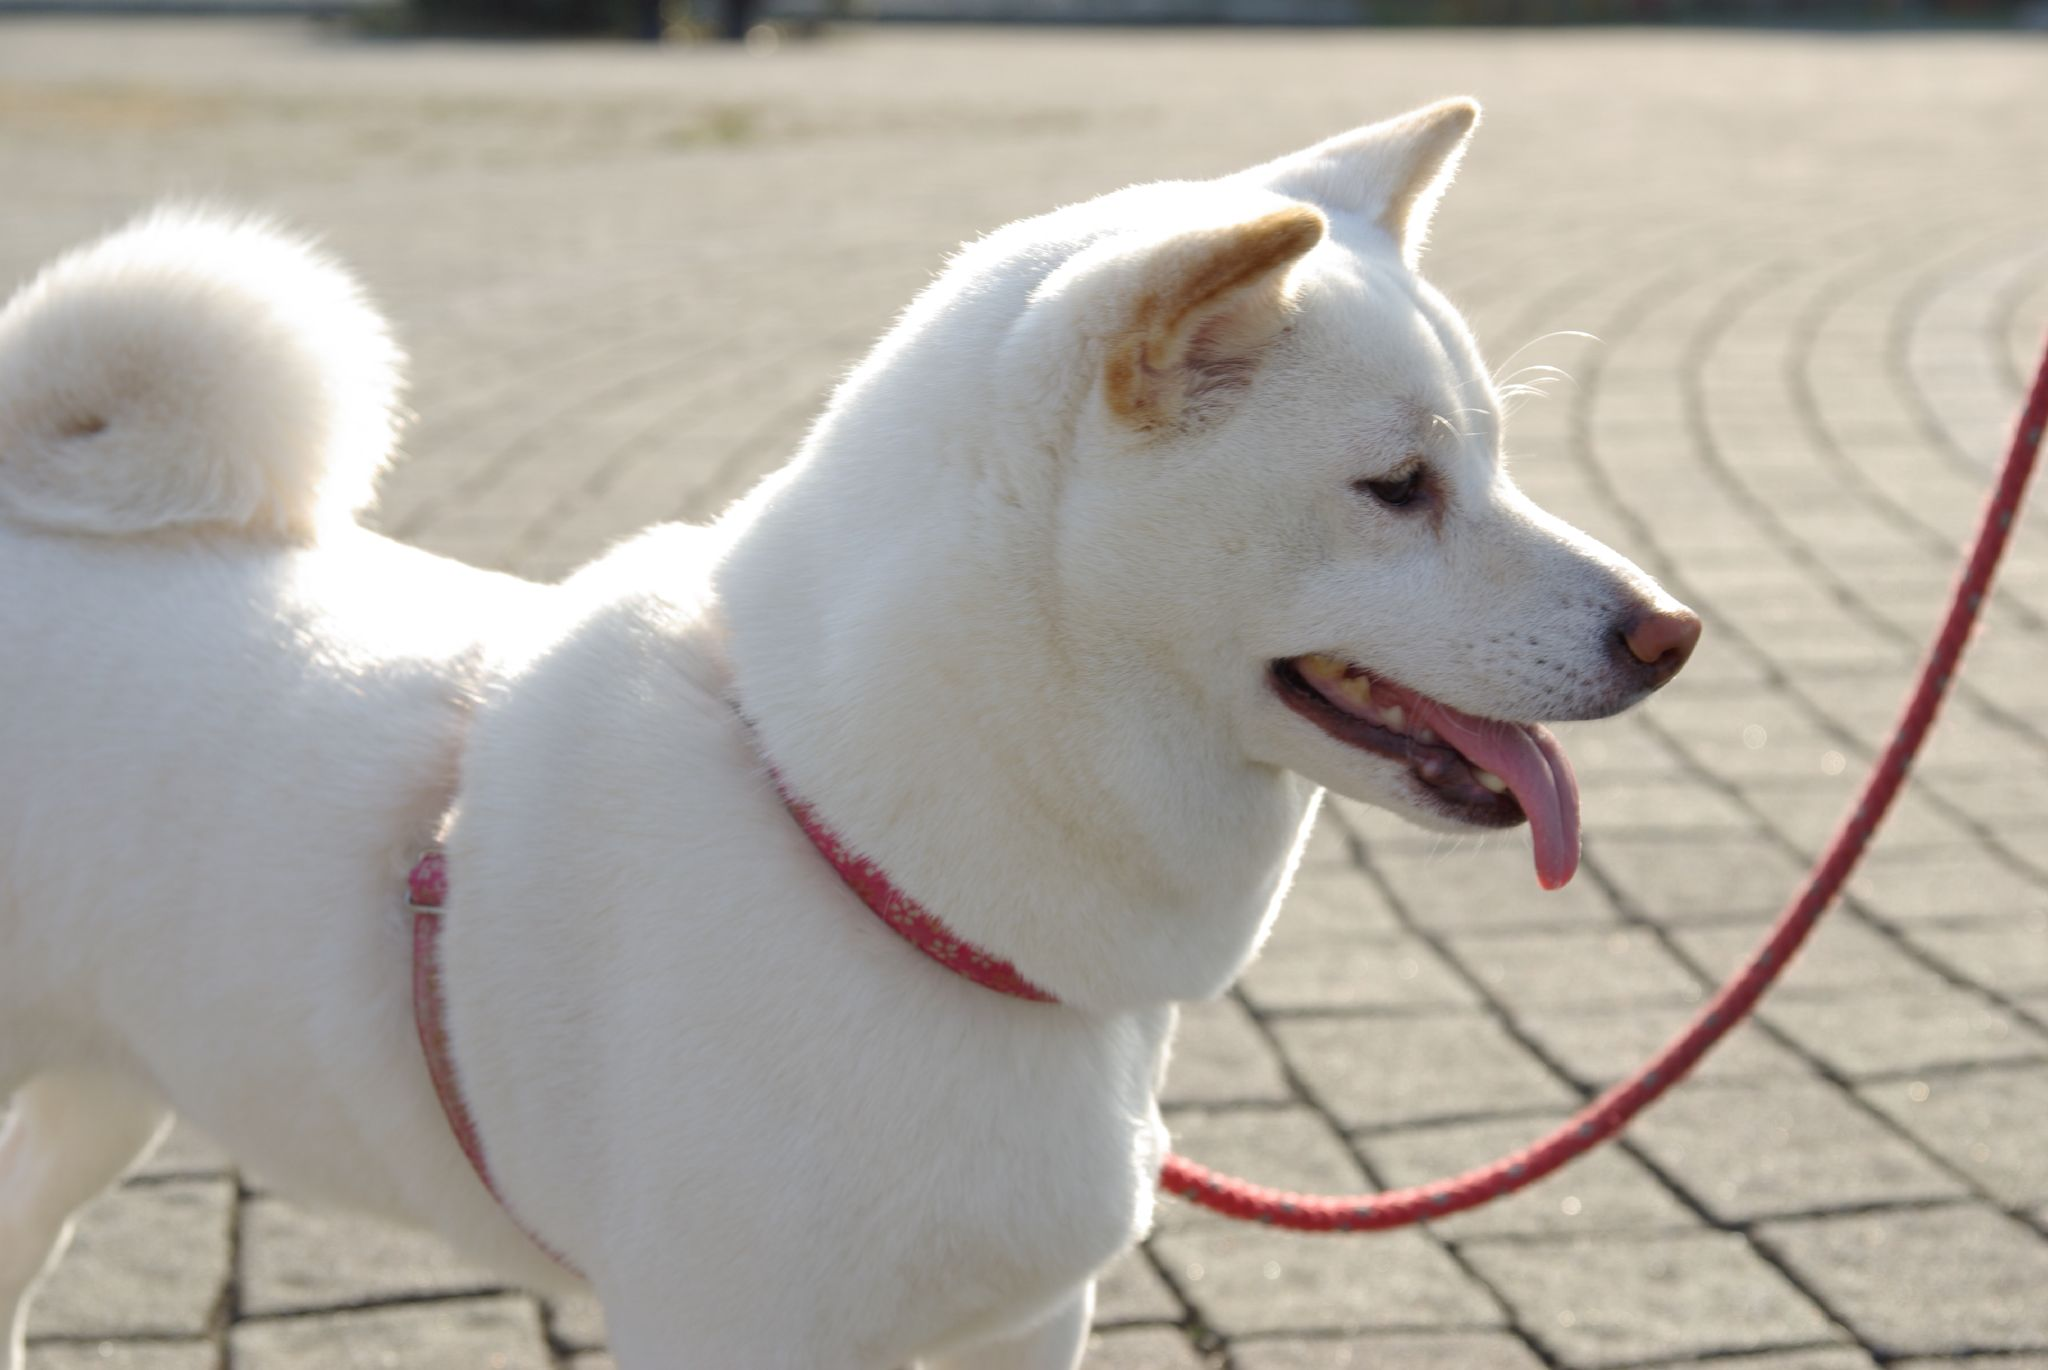
\includegraphics[width=8cm]{shiba.jpg}
\caption{A picture of a good boy.}
\label{fig:doggo}
\end{figure}
%
\section*{Lorem ipsum}
%
\lipsum[1-6] \par
%
\section*{Japanese sample text}
%
いづれの御時にか、女御、更衣あまたさぶらひたまひけるなかに、いとやむごとなき際にはあらぬが、すぐれて時めきたまふありけり。
はじめより我はと思ひ上がりたまへる御方がた、めざましきものにおとしめ嫉みたまふ。同じほど、それより下臈の更衣たちは、ましてやすからず。朝夕の宮仕へにつけても、人の心をのみ動かし、恨みを負ふ積りにやありけむ、いとあつしくなりゆき、もの心細げに里がちなるを、いよいよあかずあはれなるものに思ほして、人の そしりをもえ憚らせたまはず、世のためしにもなりぬべき御もてなしなり。
上達部、上人なども、あいなく目を側めつつ、「いとまばゆき人の御おぼえなり。唐土にも、かかる事の起こりにこそ、世も乱れ、あしかりけれ」と、やうやう天の下にもあぢきなう、人のもてなやみぐさになりて、楊貴妃の例も引き出でつべくなりゆくに、いとはしたなきこと多かれど、かたじけなき御心ばへのたぐひなきを頼みにてまじらひたまふ。
父の大納言は亡くなりて、母北の方なむいにしへの人のよしあるにて、親うち具し、さしあたりて世のおぼえはなやかなる御方がたにもいたう劣らず、なにごとの儀式をももてなしたまひけれど、とりたててはかばかしき後見しなければ、事ある時は、なほ拠り所なく心細げなり。
先の世にも御契りや深かりけむ、世になく清らなる玉の男御子さへ生まれたまひぬ。いつしかと心もとながらせたまひて、急ぎ参らせて御覧ずるに、めづらかなる稚児の御容貌なり。
一の皇子は、右大臣の女御の御腹にて、寄せ重く、疑ひなき儲けの君と、世にもてかしづききこゆれど、この御にほひには並びたまふべくもあらざりければ、おほかたのやむごとなき御思ひにて、この君をば、私物に思ほしかしづきたまふこと限りなし。
初めよりおしなべての上宮仕へしたまふべき際にはあらざりき。おぼえいとやむごとなく、上衆めかしけれど、わりなくまつはさせたまふあまりに、さるべき御遊びの折をり、何事にもゆゑある事のふしぶしには、まづ参う上らせたまふ。ある時には大殿籠りすぐして、やがてさぶらはせたまひなど、あながちに御前去らずもてなさせたまひしほどに、おのづから軽きかたにも見えしを、この御子生まれたまひてのちは、いと心ことに思ほしおきてたれば、坊にも、ようせずは、この御子の居たまふべきなめりと、一の皇子の女御はおぼし疑へり。人より先に参りたまひて、やむごとなき御思ひなべてならず、皇女たちなどもおはしませば、この御方の御いさめをのみぞ、なほわづらはしう心苦しう思ひきこえさせたまひける。
かしこき御蔭をば頼みきこえながら、おとしめ疵を求めたまふ人は多く、わが身はか弱くものはかなきありさまにて、なかなかなるもの思ひをぞしたまふ。御局は桐壷なり。あまたの御方がたを過ぎさせたまひて、ひまなき御前渡りに、人の御心を尽くしたまふも、げにことわりと見えたり。参う上りたまふにも、あまりうちしきる折をりは、打橋、渡殿のここかしこの道に、あやしきわざをしつつ、御送り迎への人の衣の裾、堪へがたく、まさなきこともあり。またある時には、え避らぬ馬道の戸を鎖しこめ、こなたかなた心を合はせて、はしたなめわづらはせたまふ時も多かり。事にふれて数知らず苦しきことのみまされば、いといたう思ひわびたるを、いとどあはれと御覧じて、後涼殿にもとよりさぶらひたまふ更衣の曹司を他に移させたまひて、上局に賜はす。その恨みましてやらむかたなし。
この御子三つになりたまふ年、御袴着ぎのこと一の宮のたてまつりしに劣らず、内蔵寮、納殿の物を尽くして、いみじうせさせたまふ。それにつけても、世の誹りのみ多かれど、この御子のおよすけもておはする御容貌心ばへありがたくめづらしきまで見えたまふを、え嫉みあへたまはず。ものの心知りたまふ人は、かかる人も世に出でおはするものなりけりと、あさましきまで目をおどろかしたまふ。
その年の夏、御息所、はかなき心地にわづらひて、まかでなむとしたまふを、暇さらに許させたまはず。年ごろ、常のあつしさになりたまへれば、御目馴れて、「なほしばしこころみよ」とのみのたまはするに、日々に重りたまひて、ただ五六日のほどにいと弱うなれば、母君泣く泣く奏して、まかでさせたてまつりたまふ。かかる折にも、あるまじき恥もこそと心づかひして、御子をばとどめたてまつりて、忍びてぞ出でたまふ。
限りあれば、さのみもえ留めさせたまはず、御覧じだに送らぬおぼつかなさを、言ふ方なく思ほさる。いとにほひやかにうつくしげなる人の、いたう面痩せて、いとあはれとものを思ひしみながら、言に出でても聞こえやらず、あるかなきかに消え入りつつものしたまふを御覧ずるに、来し方行く末思し召されず、よろずのことを泣く泣く契りのたまはすれど、御いらへもえ聞こえたまはず、まみなどもいとたゆげにて、いとどなよなよと、我かの気色にて臥したれば、いかさまにと思し召しまどはる。輦車の宣旨などのたまはせても、また入らせたまひて、さらにえ許させたまはず。
% ----------------------------------------------------
% ---                BODY ENDS HERE                ---
% ----------------------------------------------------
\printbibliography
%
\end{document}